%------------------------------------------------
\section{Surface d'Attaque}
%------------------------------------------------

\begin{frame}
\begin{columns}
\column{0.5\textwidth}
\begin{itemize}
    \item La surface d'attaque est un concept permettant d'évaluer le risque auquel est exposé un système informatique.
    \item Un ordinateur sans connexion Internet est dit "Air-Gapped"
\end{itemize}
\column{0.5\textwidth}
Ordinateur sans connexion Internet: quelle est la surface d'attaque?
\begin{figure}
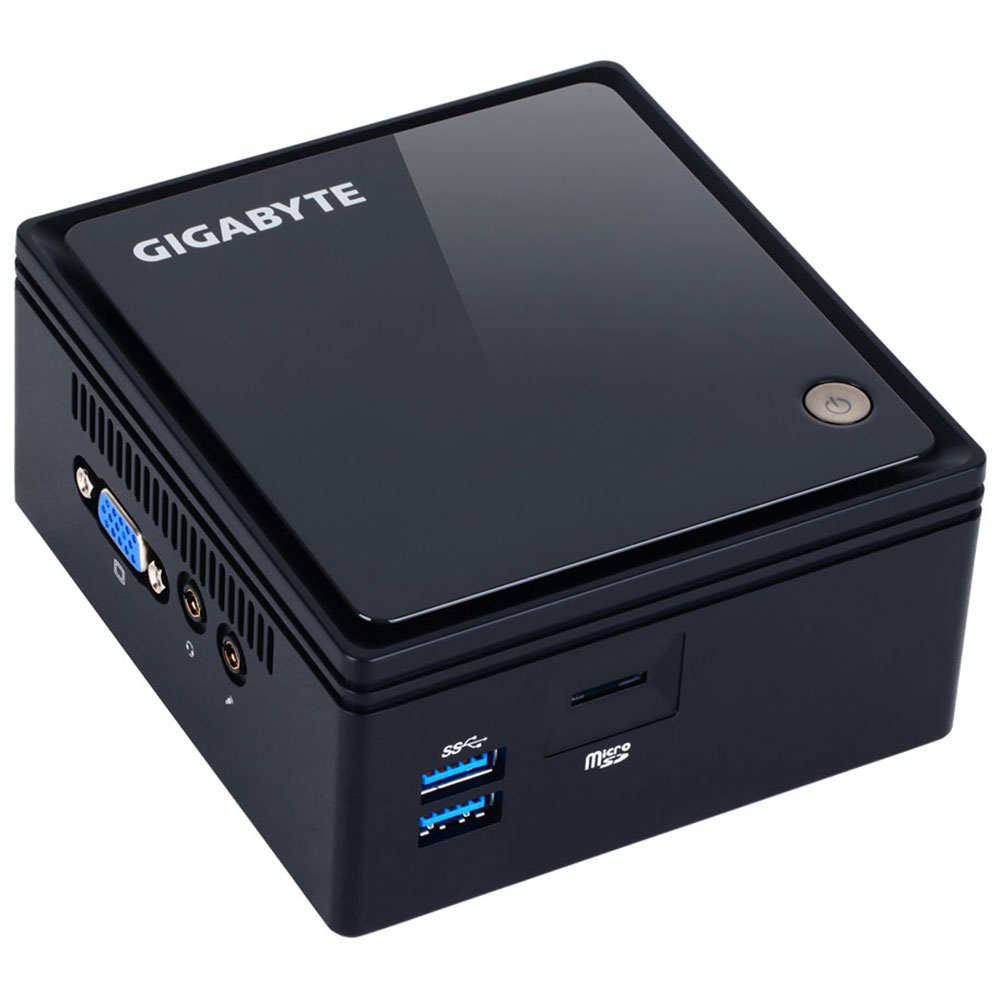
\includegraphics[scale=0.15]{res/brix}
\end{figure}
 
\end{columns}


\end{frame}
%------------------------------------------------

\begin{frame}
\begin{columns}
\column{0.5\textwidth}
\begin{itemize}
    \item La surface d'attaque est un concept permettant d'évaluer le risque auquel est exposé un système informatique.
    \item Un ordinateur sans connexion Internet est dit "Air-Gapped"
\end{itemize}
\column{0.5\textwidth}
Ordinateur sans connexion Internet: quelle est la surface d'attaque?
\begin{figure}
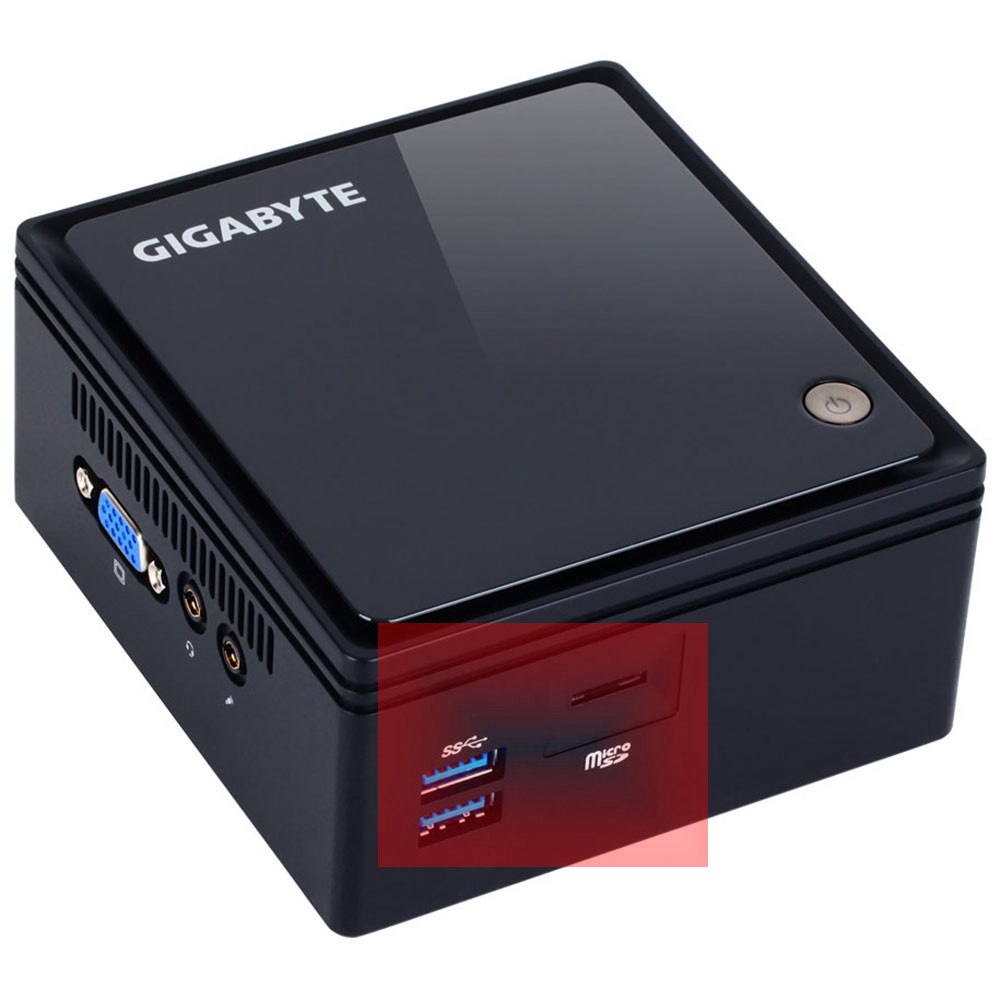
\includegraphics[scale=0.15]{res/brix2}
\end{figure}
Les ports USB.
\end{columns}


\end{frame}
%------------------------------------------------

\begin{frame}

L'USB c'est cool:
\begin{itemize}
    \item On branche une clef USB -> ça marche !
    \item On branche un clavier USB -> ça marche !
    \item Est-ce que une clef USB peut prétendre être un clavier ?
    \begin{itemize}
        \item Ouaip.
    \end{itemize}
\end{itemize}

\begin{figure}
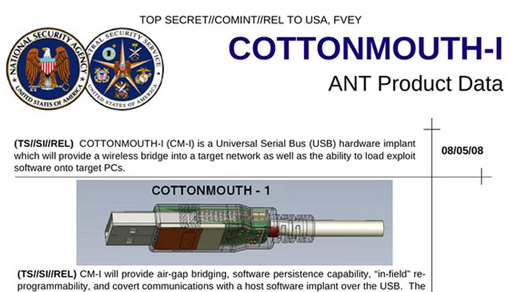
\includegraphics[scale=0.55]{res/badusb}
\end{figure}


\end{frame}

%------------------------------------------------

\begin{frame}
\begin{center}
Serveur connecté à internet, sans services.

\begin{itemize}
    \item Les ports Physiques (USB etc)
    \item Le driver réseau
    \item La fonction de routage du Kernel
\end{itemize}

+ serveur SSH.

\begin{itemize}
    \item Les ports Physiques (USB etc)
    \item Le driver réseau
    \item La fonction de routage du Kernel
    \item Le serveur SSH
\end{itemize}
\end{center}

\end{frame}



%------------------------------------------------
\begin{frame}

Station de travail sous Windows avec un antivirus connectée à internet, avec un employé qui consulte Facebook
\begin{itemize}
    \item Les ports Physiques (USB etc)
    \item Le driver réseau
    \item La fonction de routage du Kernel
    \item L'antivirus
    \item Le navigateur web
\end{itemize}

\end{frame}



%------------------------------------------------


\begin{frame}

Pour analyser la surface d'attaque, vous devez:
\begin{itemize}
    \item Noter tous les flux de données extérieures dans votre SI
    \item Recenser tout le matériel soumis à ces flux de données
    \item Recenser toute la couche logicielle soumis à ces flux de données
\end{itemize}

\end{frame}




